\documentclass[a4paper,ngerman,12pt]{scrartcl}

\usepackage[utf8]{inputenc}
%\usepackage[ansinew]{inputenc}

\usepackage[ngerman]{babel}

\usepackage{amsmath,amsthm,amssymb,stmaryrd,color,graphicx}
\usepackage{setspace}
\usepackage{bussproofs}
\usepackage{array}
\usepackage{comment}

\usepackage{enumitem}

\usepackage[protrusion=true,expansion=true]{microtype}

\usepackage{lmodern}

\usepackage{hyperref}
\usepackage{cleveref}

\newcommand{\RR}{\mathbb{R}}
\newcommand{\CC}{\mathbb{C}}
\newcommand{\ZZ}{\mathbb{Z}}
\newcommand{\NN}{\mathbb{N}}
\newcommand{\QQ}{\mathbb{Q}}

\setlength\parskip{\medskipamount}
\setlength\parindent{0pt}

\theoremstyle{definition}
\newtheorem{defn}{Definition}[]
\newtheorem{axiom}[defn]{Axiom}
\newtheorem{bsp}[defn]{Beispiel}

\theoremstyle{plain}
\newtheorem{prop}[defn]{Proposition}
\newtheorem{motto}[defn]{Motto}
\newtheorem{wunder}[defn]{Wunder}
\newtheorem{ueberlegung}[defn]{Überlegung}
\newtheorem{lemma}[defn]{Lemma}
\newtheorem{kor}[defn]{Korollar}
\newtheorem{hilfsaussage}[defn]{Hilfsaussage}
\newtheorem{satz}[defn]{Satz}

\theoremstyle{remark}
\newtheorem{bem}[defn]{Bemerkung}
\newtheorem{aufg}[defn]{Aufgabe}

\newlength{\aufgabenskip}
\setlength{\aufgabenskip}{1.4em}
\newcounter{aufgabennummer}
\newenvironment{aufgabe}[1]{
  \addtocounter{aufgabennummer}{1}
  \textbf{Aufgabe \theaufgabennummer.} \emph{#1} \par
}{\vspace{\aufgabenskip}}

\clubpenalty=10000
\widowpenalty=10000
\displaywidowpenalty=10000

\setlength\unitlength{1cm}

\usepackage{tikz}
\def\mkPascal#1{
  \begin{tikzpicture}
    \def\dx{20pt}
    \def\dy{30pt}
    \newcounter{i}
    \stepcounter{i}
    \node (\arabic{i}) at (0,0) {1};
    \foreach [count=\i] \x in {2,...,#1}{
      \pgfmathsetmacro{\lox}{\x-1}%
      \pgfmathsetmacro{\loxt}{\x-3}%
      \foreach [count=\j] \xx in {-\lox,-\loxt,...,\lox}{
        \pgfmathsetmacro{\jj}{\j-1}%
        \stepcounter{i}
        \pgfmathsetmacro{\lbl}{\lox!/(\jj!*(\lox-\jj)!)}
        \node  (\arabic{i}) at (\xx*\dx, -\lox*\dy) {\pgfmathint{\lbl}\pgfmathresult};
      }
    }
    \newcounter{z}
    \newcounter{xn}
    \newcounter{xnn}
    \pgfmathsetmacro{\maxx}{#1 - 1}
    \foreach \x in {1,...,\maxx}{
      \foreach \xx in {1,...,\x}{
        \stepcounter{z}
        \setcounter{xn}{\arabic{z}}
        \addtocounter{xn}{\x}
        \setcounter{xnn}{\arabic{xn}}
        \stepcounter{xnn}
          \draw [->] (\arabic{z}) -- (\arabic{xn});
          \draw [->] (\arabic{z}) -- (\arabic{xnn});
      }
    }
  \end{tikzpicture}
}

\RequirePackage{geometry}
\geometry{textwidth=16.0cm,textheight=24.5cm,footskip=1.5cm}

\begin{document}

\begin{picture}(0,0)
  \put(0,-0.5){%
    
\includegraphics[scale=0.1]{logo-ifm}
  }
  \put(14.0,-3.5){%
    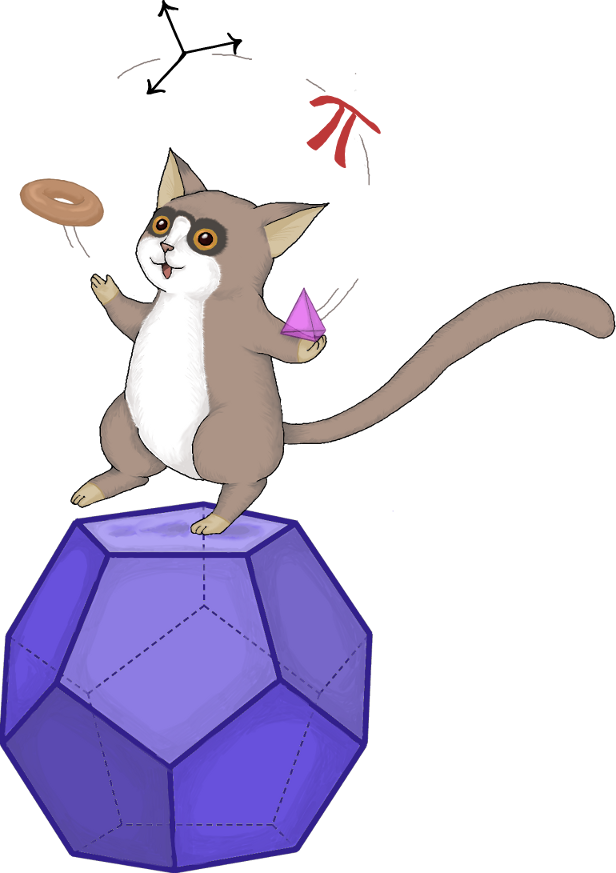
\includegraphics[scale=0.17]{cover}
  }
\end{picture} 

\vspace{6em}

\begin{center}\Large{Dritter Korrespondenzbrief}\end{center}

\section*{Fraktale Dimensionen}

Einleitung!


\section{Die Kochsche Schneeflocke}

\section{Dimensionen}


\begin{defn}
Definition der Fraktalen Dimension\footnote{Tatsächlich gibt es mehrere Möglichkeiten fraktale Dimensionen zu definieren - wir betrachten hier die sogenannte \glqq Ähnlichkeits-Dimension\grqq{}}
\end{defn}

\begin{bem}
Logarithmus mit Taschenrechner berechnen
\end{bem}

\section{Mehr Fraktale}

Sirpinski-Dreieck (Erinnerung an Pascalsches Dreieck!)

evtl. Menger-Schwamm

evtl. Drachenkurve (Basteln!)

\section{Fraktale im echten Leben}

Küstenlinie messen?

\end{document}
